%%%%%%%%%%%%%%%%%%%%%%%%%%%%%%%%
\chapter{Definição dos Modelos}%
%%%%%%%%%%%%%%%%%%%%%%%%%%%%%%%%

O cálculo do \textit{PageRank} possui desde um modelo mais simples, até outras adaptações deste modelo devido aos problemas descritos no capítulo anterior. A estimação do \textit{PageRank} é feita por uma equação de diferença, a qual possui uma matriz de transição do tipo estocástica. Na primeira seção deste capítulo é demostrada a construção dessa matriz. Na sequência são apresentados o \textit{Power Method}, modelo mais simples do cálculo do \textit{PageRank}, o \textit{Teleportation Model}, modelo que trata da navegação descontínua e o modelo por trás dos algoritmos distribuídos.   


%%%%%%%%%%%%%%%%%%%%%%%%%%%%%%%%%%%%%%
\section{A Matriz \textit{Hyperlink}}%
%%%%%%%%%%%%%%%%%%%%%%%%%%%%%%%%%%%%%%

A construção da matriz \textit{hyperlink} é feita com base na estrutura da \textit{Web}, ou ainda do grafo que a representa. Assim, considerando que o grafo da figura \ref{grafo} representa um conjunto de páginas interligadas, seus elementos são definidos da seguinte forma: 

\
\begin{figure}[!htb]
	\centering
	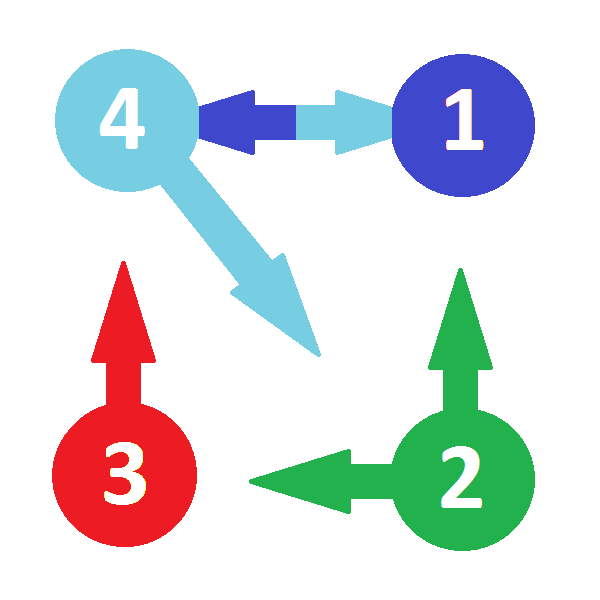
\includegraphics[scale=0.4]{imagens/grafo}
	\caption{Grafo representando \textit{links} entre páginas \textit{Web}.}
	\label{grafo}
\end{figure}

\begin{itemize}
\item $n$: como os n\'os, que representam as p\'aginas,

\vspace{0.1cm}
	
\item $\mathcal{E}$: como as arestas, que representam os \textit{links} entre as páginas.
\end{itemize}

Para representar o \textit{link} entre duas páginas específicas usa-se $i$ e $j$, de forma que o $i$ esteja associado à página de saída e $j$ com a de entrada. Considerando então o caso de um v\'ertice $i$ estar conectado a um $j$, tem-se $(i,j) \in \mathcal{E}$.

A matriz de transição que é construída a partir do grafo tem a seguinte propriedade para cada um de seus elementos:

\begin{equation}\label{a}
a_{ij} = \begin{cases}
\dfrac{1}{n_i}, & \text{caso}\, (i,j)\in \mathcal{E},\\
0, & \text{caso contr\'ario}.
\end{cases}
\end{equation}	

Cada elemento $a_{ij}$ é formado a partir das relações entre os nós do grafo. Para o nó $1$ por exemplo, constata-se que ele só possui relações com o nó $4$, por tanto, para um navegador que encontra-se em $1$ tem-se $100\%$, de certeza de que seu próximo passo será para $4$. Já no caso do nó $2$ pode-se observar que o navegador pode ir para $1$ ou $3$, ou seja, ele tem $50\%$ de chance de ir para cada um desses dois nós.

\begin{equation}\label{A}
A = \begin{pmatrix}
 0 & 1/2 & 0 & 1/2 \\
 0 &  0  & 0 & 1/2 \\
 0 & 1/2 & 0 &  0  \\
 1 &  0  & 1 &  0
\end{pmatrix}
\end{equation}

E assim constroi-se a matriz de transição \eqref{A} de forma que todas as suas colunas respeitem a propriedade:

\begin{equation}\label{n}
\sum^{n}_{i=1} x_{i} = 1.
\end{equation}

Vale ressaltar que partindo de qualquer nó, todos os outros nós ligados a este possuem a mesma probabilidade de serem acessados. Ou seja, em uma página um \textit{link} ou outro não terão maior probabilidade de serem acessados por chamarem mais atenção, ou por qualquer outro motivo.

Sendo assim, o grafo, ou o conjunto de páginas, trata-se de uma cadeia de Markov com espaço de estados de dimensão $n$. Onde a estimação de uma posição seguinte apenas depende da atual.

%, seguindo a propriedade de Markov \ref{p}.

%\begin{equation}\label{p}
%P \bigl( \theta(k+1) = j \mid  \theta(k) = i_k, \theta(k-1) = i_{k-1}, \ldots, \theta(0) = i_0\bigr) = P %\bigl( \theta(k+1) = j \mid  \theta(k) = i_k\bigr).
%\end{equation}


%%%%%%%%%%%%%%%%%%%%%%%%%%%%%%%%%%
\section{O \textit{Power Method}}%
%%%%%%%%%%%%%%%%%%%%%%%%%%%%%%%%%%

Este é o modelo mais simples para a estimação do \textit{PageRank}. Esta abordagem constitui-se de uma equação de diferença, a qual possui uma matriz de transição coluna estocástica e um vetor estocástico. O vetor estocástico é formado pelos valores das variáveis aleatórias da cadeia de Markov, ou seja, os valores das páginas. O valor de \textit{PageRank} de um conjunto de $n$ páginas da \textit{Web} é definido como o vetor $x \in \mathbb{R}^{n \times 1}$ que satisfaz as seguintes equações:

\begin{equation}	
x = Ax, \quad x\geq0, \quad \sum^{n}_{i=1} x_{i} = 1, 
\end{equation}

\noindent onde $A \in \mathbb{R}^{n \times n}$ é a transposta da matriz de transição da cadeia de Markov.

Assim, o método usual para obtenção do \textit{PageRank} é o chamado \textit{Power Method} \cite{ishii2014pagerank}, que alcança o \textit{PageRank} através da seguinte iteração:

\begin{equation}
x(k+1) = Ax(k), \quad k\geq0, \quad \text{com} \quad x(0) = x_0,
\end{equation}

\noindent onde $x_0 \in \mathbb{R}^{n \times 1}$ é uma condição inicial positiva de soma igual a um.


%%%%%%%%%%%%%%%%%%%%%%%%%%%%%%%%%%%%%%%%%%%%%%%%%%%%%%%%%%%%%%
\subsection{Questões de Convergência do \textit{Power Method}}%
%%%%%%%%%%%%%%%%%%%%%%%%%%%%%%%%%%%%%%%%%%%%%%%%%%%%%%%%%%%%%%

Após um número considerável de iterações e em um número considerável de casos, o \textit{Power Method} atinge a distribuição limite com os valores de \textit{PageRank} de cada página. Além disso, independente da condição inicial, ao final das iterações os valores de \textit{PageRank} tendem a ser os mesmos.

Isso ocorre devido a matriz de transição ser irredutível, o que reflete no navegador aleatório sempre conseguir chegar a uma certa página partindo de uma outra qualquer, mesmo que essas duas páginas não estejam diretamente conectadas. Observando o grafo da figura \ref{grafo}, pode-se observar que não existe um \textit{link} direto entre $1$ e $3$, para chegar-se em $3$ a partir de $1$ o usuário teria de ir de $1$ para $4$, de $4$ para $2$ e de $2$ para $3$.

No caso de uma página apenas possuir \textit{links} de entrada, como por exemplo, ao acessar-se um documento PDF, o problema é contornado ao admitir-se que o usuário poderia usar o botão de voltar do \textit{Browser}, criando um \textit{link} de saída da página. Assim, a matriz mantem-se irredutível, garantindo que para a maioria das condições iniciais os valores de \textit{PageRank} sejam os mesmos ao atingir-se a distribuição limite. No entanto, existem alguns casos em que não há garantia de convergência, e por tanto o modelo do \textit{Power Method} tem de sofrer algumas alterações. 


%%%%%%%%%%%%%%%%%%%%%%%%%%%%%%%%%%%%%%%%%
\section{O \textit{Teleportation Model}}%
%%%%%%%%%%%%%%%%%%%%%%%%%%%%%%%%%%%%%%%%%

O valor de \textit{PageRank} é estimado após inúmeras iterações entre o vetor de valores das páginas e a matriz de transição estocástica. No entanto mesmo observando os valores das páginas em um grande horizonte de tempo, existem casos em que eles não convergem. O modelo do \textit{Power Method} é atraente pela sua simplicidade, entretanto alguns problemas fazem com que ele não ofereça uma garantia de convergência. O maior desses problemas é devido a possibilidade do usuário fazer uma navegação descontínua no grafo, em que ele saltaria de uma página para outra, de forma a não seguir a estrutura de \textit{links} da rede. Todavia, existe um modelo para resolver o problema da navegação com saltos, modelo este conhecido como \textit{Teleportation Model}. 

O \textit{Teleportation Model} é uma estratégia reconhecida para que, através de uma pequena modificação na matriz $A$, o método convirja globalmente para o PageRank. Essa modificação na matriz $A$ é representada como uma combinação convexa de duas matrizes, em que a matriz de transição agora passa a ser $M$, dada por:

\begin{equation}
M = (1-m)A + \frac{m}{n}{\bf11}^T,
\end{equation}

\noindent onde $M \in \mathbb{R}^{n \times n}$, $m \in (0,1)$ e $\textbf{1} \in \mathbb{R}^{N \times 1}$. Em que $\textbf{11}^T$ é uma matriz preenchida de 1's, resultante do produto entre um vetor de 1's $\textbf{1}$ e um vetor de 1's transposto $\textbf{1}^T$. Vale lembrar também que $n$ é o número de nós do grafo, ou número de páginas, e que $A$ continua sendo a mesma matriz de transição, apenas é substituida por $M$ na equação apresentada no \textit{Power Method}.


%%%%%%%%%%%%%%%%%%%%%%%%%%%%%%%%%%%%%%%%%%%%%%%%%
\section{O Modelo dos Algoritmos Distribu\'idos}%
%%%%%%%%%%%%%%%%%%%%%%%%%%%%%%%%%%%%%%%%%%%%%%%%%

Por fim, um último problema é considerado antes de serem feitas as simulações, a massividade da \textit{Web}. O fato da \textit{internet} ter um grande número de páginas, faz com que o tempo necessário para o cálculo e ranqueamento das páginas seja extremamente grande. A fim de tornar o cálculo do \textit{PageRank} menos custoso, e melhor explorar os recursos computacionais dos servidores disponíveis na web, uma alternativa é o emprego de algoritmos distribuídos. A agregação de tais experimentos aleatórios faz então com que o \textit{power method} se torne um sistema linear com saltos Markovianos do seguinte tipo:

\begin{equation}
	x(k+1) = A_{\theta(k)}x(k), \quad k\geq0, \quad \text{com} \quad x(0) = x_0. 
\end{equation}

Em que a matriz de transição $A$ agora passa a ser várias matrizes \textit{links} distribu\'idas $A_i \in \mathbb{R}^{n \times n}, \: i = 1,2, ..., n$. Sendo cada uma das matrizes distribuídas definidas da seguinte forma: 

\begin{itemize}
\item a i-ésima coluna de $A_i$ coincide com a i-ésima coluna de $A$,
\item a j-ésima entrada diagonal de $A_i$ é igual a um para $j = 1, ..., n, \: j \neq i$,
\item todas as outras entradas $a_{ij}$ são iguais a zero.
\end{itemize}

A ideia agora é de que cada página fará o seu cálculo de \textit{PageRank}, por isso são criadas as matrizes  distribuídas. Com relação a construção das matrizes, pode-se observar que elas seguem a seguinte ideia. As colunas das matrizes são formadas pelas relações de saída de cada um dos nós, ao mesmo tempo que cada matriz \textit{link} distribuída está associada a um nó do grafo da figura \ref{grafo}. Assim a coluna $1$ de $A$ \eqref{A} é copiada para a primeira coluna de $A_1$ \eqref{A12}, o restante da diagonal pricipal é preenchida com 1's e o restante dos elementos é zero. O mesmo se repete para as outras matrizes distribuídas.

\begin{equation}\label{A12}
A_1 = \begin{pmatrix}
 0 &  0  & 0 &  0 \\
 0 &  1  & 0 &  0 \\
 0 &  0  & 1 &  0  \\
 1 &  0  & 0 &  1
\end{pmatrix}
%
\hspace{0.5cm}
%
A_2 = \begin{pmatrix}
 1 & 1/2 & 0 &  0 \\
 0 &  0  & 0 &  0 \\
 0 & 1/2 & 1 &  0  \\
 0 &  0  & 0 &  1
\end{pmatrix}
\end{equation}

\vspace{0.1cm}

\begin{equation}\label{A34}
A_3 = \begin{pmatrix}
 1 &  0  & 0 &  0 \\
 0 &  1  & 0 &  0 \\
 0 &  0  & 0 &  0  \\
 0 &  0  & 1 &  1
\end{pmatrix}
%
\hspace{0.5cm}
%
A_4 = \begin{pmatrix}
 1 &  0  & 0 & 1/2 \\
 0 &  1  & 0 & 1/2 \\
 0 &  0  & 1 &  0  \\
 0 &  0  & 0 &  0
\end{pmatrix}
\end{equation}	

Acoplando agora o modelo das matrizes distribuídas ao modelo do \textit{Teleportation} tem-se \eqref{Ax},

\begin{equation} \label{Ax}
x(k+1) = (1 - \hat{m})A_{\theta(k)}x(k) + \frac{\hat{m}}{n} \textbf{1}, \quad k \geq 0, \quad \text{com} \quad x(0) = x_0,
\end{equation}

\noindent onde $\hat{m}$ é definido como: 

\begin{equation}\label{m}
\hat{m} = \frac{2m}{n-m(n-2)},
\end{equation}

\noindent e $m = 0.15$, é um parâmetro que foi obtido através de testes em \cite{zaki2012detection}.    

%%%%%%%%%%%%%%%%%%%%%%%%%%%%%%%%%%%%%%%%%%%%%%%%%%%%%%%%%%%%
\subsection{Questões de Convergência do Modelo Distribuído}%
%%%%%%%%%%%%%%%%%%%%%%%%%%%%%%%%%%%%%%%%%%%%%%%%%%%%%%%%%%%%

De forma similar ao que ocorre no \textit{Power Method}, este método apresenta problemas de convergência, pois as matrizes $A_1$, $A_2$, $A_3$ e $A_4$ não são irredutíveis. Isso ocorre devido a inserção de 1's nas diagonais, o que na prática implicaria no nó $4$ só ter saída e chegada nele mesmo. Dessa forma, usando-se da matriz $A_1$, por exemplo, um navegador aleatório que partisse de $4$, nunca sairia de lá.

Para isso é usada uma média no tempo, em que a cada iteração é feita uma média de todos os estados anteriores. Assim $y(k)$ é a média do conjunto de amostras $x(0),... , x(k)$ definida como \eqref{y}, 

\begin{equation}\label{y}
y(k) = \frac{1}{k+1} \sum_{l=0}^{k} x(l).
\end{equation}

%De tal forma que o algoritmo converge no sentido da média quadrática \eqref{E}, em que quanto maior é o número de iterações $k$, mais o valor se aproxima da distribuição limite, ou seja, do valor de \textit{PageRank}. 

\noindent De tal forma que o algoritmo converge no sentido da média quadrada, ou seja,

\begin{equation}\label{E}
\lim_{k\rightarrow \infty} \mathbb{E} [\parallel y(k)-x^*\parallel^2] = 0.
\end{equation}

\noindent Neste contexto, quanto maior for o número de iterações $k$, mais o valor de $y(k)$ se aproxima da
distribuição limite, o que representa o valor de \textit{PageRank}.

A fim de minimizar custos computacionais, um formato recursivo da média $y(k)$ foi usado nas simulações, que possui o seguinte formato:

\begin{equation}\label{yr}
	y(k+1) = \frac{(k+1)}{(k+2)}y(k) + \frac{1}{(k+2)}x(k+1).
\end{equation}

%Por que essa estratégia diminui o custocomputacional?
A média em seu formato recursivo \eqref{yr} diminui o custo computacional pois a cada nova iteração do vetor $y(k)$ apenas leva-se em conta o seu estado anterior $y(k-1)$. A média em seu formato comum \eqref{y} é estimada a cada nova iteração a partir de todos os outros estados anteriores, o que eleva consideravelmente o custo computacional. A dedução do modelo recursivo da média é apresentado no Apêndice A.